\documentclass{article}
\usepackage[utf8]{inputenc}

% trees
\usepackage{tikz}
\usetikzlibrary{trees}

% for the thumbs
\usepackage{fontawesome}

% arrows with text
\usepackage{mathtools}

% block comments
\usepackage{comment}

% nested bullet itemize
\usepackage{enumitem}

% pddl code blocks
\usepackage{listings}
\lstdefinelanguage{PDDL}
{
  sensitive=false,    % not case-sensitive
  morecomment=[l]{;}, % line comment
  alsoletter={:,-},   % consider extra characters
  morekeywords={
    define,domain,problem,not,and,or,when,forall,exists,either,
    :domain,:requirements,:types,:objects,:constants,
    :predicates,:action,:parameters,:precondition,:effect,
    :fluents,:primary-effect,:side-effect,:init,:goal,
    :strips,:adl,:equality,:typing,:conditional-effects,
    :negative-preconditions,:disjunctive-preconditions,
    :existential-preconditions,:universal-preconditions,:quantified-preconditions,
    :functions,assign,increase,decrease,scale-up,scale-down,
    :metric,minimize,maximize,
    :durative-actions,:duration-inequalities,:continuous-effects,
    :durative-action,:duration,:condition
  }
}

\title{Planning}
\author{Daniel Gigliotti}
\date{}

\begin{document}

\maketitle

\section{Search vs Planning}

% Search and planning are both methods used in artificial intelligence (AI) to achieve a goal or solve a problem. \\

Search is a method used to find a solution among a set of possibilities. It involves exploring a set of states or configurations, and using a set of rules or heuristics to determine which ones to explore next, until a goal state is found. \\

Planning, on the other hand, is a method used to determine a sequence of actions that will lead to a goal state. It involves representing the problem as a set of actions and their effects, and using a planning algorithm to determine the optimal sequence of actions to achieve the goal. \\

Planning is another approach to search but instead of having a representation which is like a black box (specific for every problem) we have a \textbf{factor representation} (it takes a specific form). Furthermore, in planning actions are specified by defining preconditions and effects; this is more scalable: if we want to introduce a new capability we just need to define a new action (add the action description) and the rest will be the same. \\

\textbf{Factor representation}: the representation is simply done by a set of variables with a finite domain of discrete values.\\ 

Planning becomes effective over search when the state space becomes too large and complex. 

\begin{itemize}
    \item \textbf{State space}: each node represents a state of the real world and a transition between nodes is an addition of an action in the action-sequence to reach a goal;
    \item \textbf{Plan space}: each node represents a partial plan; when we cross an arc we add an action from the action-set to the partial plan.
\end{itemize}

A \textbf{planning problem} is one in which we have some initial \textbf{starting state}, which we wish to transform into a desired \textbf{goal state} through the application of a set of \textbf{actions}. \\

\newpage

\begin{comment}

A \textbf{fluent} is a variable or predicate that represents a condition or state of the world in a problem domain. For example, in a robotic vacuum cleaner domain, one possible fluent could be the "location" of the vacuum cleaner and it could have different values such as "kitchen", "living room", "bedroom", etc. depending on where the vacuum cleaner is currently located. Fluents are used in planning to define the preconditions and effects of action schemas. \\

\begin{center}
    \textbf{A fluent is a condition that can change over time.}
\end{center}

A set of instantiated fluents is called a \textbf{state}. According to the \textbf{close world assumption}, a state contains only positive fluents; all the missing ones are assumed to be false. \\

\begin{center}
    \textbf{A state (factor representation) is a set of fluents.}
\end{center}

\end{comment}

\begin{itemize}
    \item \textbf{Predicates} are used to represent relationships between objects or entities. A predicate is a statement that takes one or more arguments and returns a thruth value. 

    \begin{center}
        isParentOf(x, y) \\
    
        takes two arguments and returns true if x is parent of y
    \end{center}
    \item \textbf{Fluents} are expressions of the form:

    \begin{center}
        $P(x_1, x_2, ..., x_n)$ or $\neg P(x_1, x_2, ..., x_n)$
    \end{center}
    
    where $P$ is a predicate, $0 \leq n$ and $x_i$ are either variables or constant symbols. Basically, a fluent is a predicate or the negation of a predicate.
    \item \textbf{States} are sets of instantiated fluents. Each fluent in the state represents if the corresponding property is satisfied (true) or not (false).
\end{itemize}

\textbf{Database assumption} (also known as \textbf{Close World assumption}): a state only contains positive fluents. All the missing ones are assumed to be false.

\newpage

\section{Classical planning}

A \textbf{classical planning problem} is one in which we have some initial \textbf{starting state}, which we wish to transform into a desired \textbf{goal state} through the application of a set of \textbf{actions}. We need to define 3 things:

\begin{enumerate}
    \item \textbf{States}, which are represented by sets of instantiated literals (with a boolean value or a constant);
    \item Actions or \textbf{action schema};
    \item An environment that is:
    \begin{itemize}
        \item fully observable: the agent knows everything about the environment;
        \item deterministic: the effect of each action is guaranteed;
        \item static: while the agent is thinking, nothing happens (the world does not change if the agent does not make an action and the changes happens instantly;
        \item discrete and finite;
    \end{itemize}
\end{enumerate}

Now we can model the problem as a search problem and search for the plan that leads to the goal state. Search can happen:

\begin{center}
    \begin{itemize}
        \item Forward (\textbf{progression});
        \item Backward (\textbf{regression});
        \item Using heuristics;
    \end{itemize}
\end{center}

\newpage

\section{Action Schemas}

\textbf{Action schemas} are a way to represent \textbf{actions}. Typically they includes a name, a set of preconditions, and a set of effects. The preconditions specify the conditions that must be true in the current state in order for the action to be applicable. The effects specify the changes that will be made to the state when the action is executed. \\

An action $a$ with $Preconditions(a) = q$ is \textbf{applicable} in a state $s$ iff:

\begin{itemize}
    \item every positive fluent in $q$ is in $s$;
    \item every negative fluent in $q$ is not in $s$;
\end{itemize}

\vspace{2cm}

\begin{lstlisting}[language=PDDL]
    (:action move
        :parameters ?agent ?from ?to
        :precondition( and
            (at ?agent ?from) (adj ?from ?to)
            (agent ?agent) (location ?from) (location ?to)
        )
        :effect( and
            (not (at ?agent ?from)) (at ?agent ?to)
        )
    )
\end{lstlisting}

\newpage

\section{Unification}

\textbf{Unification} of two expressions is the process of finding a substitution that, whan applied to them, makes them identical.\\

Example: ${x/b}$ is a unifier for $p(a, x)$ and $p(a, b)$ \\

Unification is applied to expressions of the form $P(t_1, t_2, ..., t_n)$. \\
$unify(P(t_1, t_2, ..., t_n), P(s_1, s_2, ..., s_n))$: find a substitution that makes $P(t_1, t_2, ..., t_n)$ and $P(s_1, s_2, ..., s_n)$ identical.

\begin{itemize}
    \item $unify(P(X), P(a)) = {X/a}$
    \item $unify(P(a), Q(a)) = ?$ (not admissible)
    \item $unify(P(X,X), P(a, b)) = ?$ (not admissible)
\end{itemize}

\newpage

\subsection{Progression}

Apply actions whose preconditions are satisfied until goal is found or all states have been explored. \\

We have to specify what is going to be the state after the execution of the action. The \textbf{effects of the action} can be positive fluents or negative fluents. 

\begin{itemize}
    \item positive fluents have to be true in the resulting state $\rightarrow$ ADD(a);
    \item negative fluents have to be false in the resulting state $\rightarrow$ DEL(a);
    \item all the fluents not in the ADD and DEL lists are kept unchanged (\textbf{persistence assumption});
\end{itemize}

\begin{center}
    Result(s, a) = (s - DEL(a)) $\cup$ ADD(a)
\end{center}

\textbf{Irrelevant} actions cause the search space to blow.

\subsection{Regression}

Search backward from the goal to the init state. If we want to go from the goal $g$ to a previous state $g'$ with an action $a$:

\begin{itemize}
    \item any positive effect of $a$ for $g$ is deleted;
    \item each precondition fluent of $a$ is added, unless it already appears;
    \item any negative effect of $a$ for $g$ is deleted from the negative literals;
    \item any negative precondition fluent of $a$ for $g$ is added to the negative literals;
\end{itemize}

\begin{center}
    POS(g') = (POS(g) - ADD(a)) $\cup$ POS(PREC(a)) \\
    NEG(g') = (NEG(g) - DEL(a)) $\cup$ NEG(PREC(a))
\end{center}

\subsection{Heuristic for planning}

Admissible heuristics can be derived from the relaxed problem which is easier to solve. Search problems can be seen as a graph where nodes are states and edges are actions. There are three ways we can relax such a problem:

\begin{itemize}
    \item \textbf{Ignoring preconditions}; this may lead to actions that achieve multiple goals (\faThumbsOUp) or to actions that undo other actions (\faThumbsODown);
    \item \textbf{Removing negated effects}; 
    \item \textbf{Decomposition}: decompose the problem into smaller, individual problems; each one will have a cost; which cost should we use for the heuristic? Should we take the max of the costs or the sum? Better do the max because maybe solving one subgoal can help solving others: summing will return a higher cost in this case, hence the heuristic is not admissible (heuristic is admissible if it does not overestimate the cost).
\end{itemize}

\newpage

\section{GraphPlan}

\textbf{Graphplan} is an efficient planning algorithm in which the data structure representing the plan is a graph. \\ 

The primary goal of Graphplan is to efficiently compute a plan for a given planning problem by representing it as a planning graph. A planning graph is a directed acyclic graph that consists of levels and layers. We have \textbf{state levels} and \textbf{action levels}. 

\begin{itemize}
    \item \textbf{State levels} contains all the literals that could be true afer the steps applied to reach that level, thus representing the state of the world;
    \item \textbf{Action levels} represent actions whose preconditions are satisfied by each state level.
\end{itemize}

State levels and action levels alternate themselves. \\

The algorithm works by incrementally expanding the planning graph, starting from an initial state and working towards a goal state. It performs two main steps in each iteration: 

\begin{itemize}
    \item the \textbf{forward search} expands the planning graph by adding new layers and propositions;
    \item the \textbf{backward search} checks for conflicts and determines if the goal state is reachable.
\end{itemize}

At each step, the algorithm tries to extract a solutiong when the goal literals appear in the last computed level and it continues until two consecutive levels are identical, i.e. the graph has \textbf{leveled off}. A literal that does not appear in the final level of the graph cannot be reached by any plan. The cost of achieving any goal literal is given by the level where it occurs in the planning graph.

\vspace{2cm}

\begin{center}
    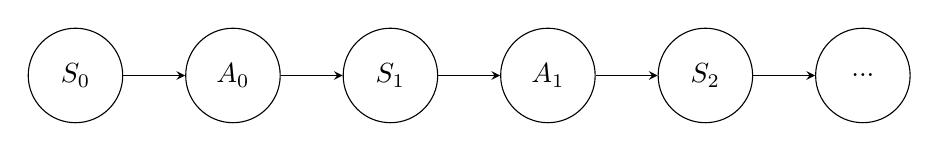
\begin{tikzpicture}
        
        \node[shape=circle, draw=black, minimum size=1.2cm] (A) at (0,0) {$S_0$};
        \node[shape=circle, draw=black, minimum size=1.2cm] (B) at (2,0) {$A_0$};
        \node[shape=circle, draw=black, minimum size=1.2cm] (C) at (4,0) {$S_1$};
        \node[shape=circle, draw=black, minimum size=1.2cm] (D) at (6,0) {$A_1$};
        \node[shape=circle, draw=black, minimum size=1.2cm] (E) at (8,0) {$S_2$};
        \node[shape=circle, draw=black, minimum size=1.2cm] (F) at (10,0) {$...$};
        
    \begin{scope}[every edge/.style={draw=black}]

        \draw [-stealth](A) edge node[left] {} (B);
        \draw [-stealth](B) edge node[left] {} (C);
        \draw [-stealth](C) edge node[left] {} (D);
        \draw [-stealth](D) edge node[left] {} (E);
        \draw [-stealth](E) edge node[left] {} (F);

    \end{scope}
        
    \end{tikzpicture}
\end{center}

\newpage

\section{Total-Order Planning (TOP)}

Forward/backward (progression/regression) state-space searches are forms of totally ordered plan search: they explore linear sequences of actions that starts with the start state and ends with the goal state, maintaining a total ordering between all actions at every stage of the planning. This way we cannot take advantages of \textbf{problem decomposition}.

\section{Partial-Order Planning (POP)}

A \textbf{partial-order plan} specifies all actions that need to be taken, but specifies an ordering between them only when necessary. This allows us to parallelize the computation (actions are often independent one from another) and we can even benefit from a situation in which we need to work on several subgoals independently: we can solve them with subplans and then put everything together. \\

\begin{itemize}
    \item Start action has the initial state description as its effects;
    \item Finish action has the goal description as its precondition;
\end{itemize}

\begin{flushleft}
    Each partial plan has four components:
\end{flushleft}

\begin{itemize}
    \item A \textbf{set of actions} that makes up the steps for the plan; an empty plan only has the Start and Finish actions;
    \item A set of \textbf{ordering constraints} between pairs of actions in the form \\ $A \prec B$;
    \item \textbf{Casual links} from outcome of one action to precondition of another \\ $A \xrightarrow{\text{p}} B$ (A achieves p for B); this is NOT the same thing as an ordering constraint;
    \item \textbf{Open preconditions}: preconditions of an action not yet casually linked;

\end{itemize}

A plan is said to be consistent if:

\begin{itemize}
    \item There are \textbf{no cycles}  e.g. $A \prec B$ and $B \prec A$;
    \item There are \textbf{no conflicts}: \\
        If we have $A \xrightarrow{\text{p}} B$ (A achieves p for B) and it exists another action $C$ that has effect $\neg p$ which undoes the effect of $A$, we have a conflict if $C$ is between $A$ and $B$. In this case, C is called a \textbf{clobber}: $A \prec C$ and $C \prec B$\\
        We can solve it by applying:
        \begin{itemize}[label=$\bullet$]
            \item \textbf{Demotion} $C \prec A$ (put the clobber before A);
            \item \textbf{Promotion} $B \prec C$ (put the clobber after B);
        \end{itemize}
\end{itemize}

\begin{flushleft}
    If in a consistent plan there is no open precondition, the plan is a \textbf{solution}.    
\end{flushleft}

\newpage

The algorithm works in the following way:

\begin{enumerate}
    \item The plan only contains $Start$ and $Finish$ with $Start\ \prec\ Finish$.
    \item The \textbf{successor function} is called:
    \begin{enumerate}
        \item pick an open condition $p$ of an action $B$;
        \item pick an action $A$ that achieves $p$;
        \item add the casual link $A \xrightarrow{\text{p}} B$ and $A \prec B$.
        \item resolve conflicts if possible, otherwise backtrack.
    \end{enumerate}
    \item The goal test succeed when there are no more open preconditions.
\end{enumerate}

POP is sound and complete: 
\begin{itemize}
    \item \textbf{sound}: if the algorithm finds a solution, the solution is correct;
    \item \textbf{complete}: if there is a solution, the algorithm will find it;
\end{itemize}

POP depends on how it chooses the action each time to fulfill the open precondition. This can be done with a suitable heuristic function.

\newpage

\section{Hierarchical Task Network Planning (HTN)}

The planning methods analyzed before all operate with a fixed set of atomic actions. This approach is not sustainable since modern problems require thousands of actions. It is important to focus on the big picture and think about the overall strategy, rather than getting bogged down in the details of individual actions. One way to do this is to use a technique called \textbf{hierarchical decomposition}, which involves \textbf{breaking down a complex problem into smaller, more manageable parts}. The key benefit of this approach is that at each level of the hierarchy, there are fewer activities to consider, which makes it easier to find the most efficient way to arrange them for the current problem. This approach can reduce the computational cost and increase the chances of success in finding the correct way to achieve the goal. \\

Planning proceeds by decomposing non-primitive tasks recursively into smaller subtasks, until primitive tasks are obtained.

\section{High-Level Actions (HLA)}

Each HLA has one or more possible refinements, into a sequence of actions, each of which may be an HLA or a primitive action. An HLA refinement that contains only primitive actions is called an \textbf{implementation} of the
HLA. We can say, then, that a \textbf{high-level plan achieves the goal from a given state if at least
one of its implementations achieve the goal from that state}.

\begin{itemize}
    \item \textbf{Primitive actions (A)} (as in classical planning) can be executed by the agent directly;
    \item \textbf{High-level actions (HLA)} cannot be executed by the agent, but have one or more \textbf{refinements} into sequences of actions.
\end{itemize}

An implementation of a \textbf{High level plan (HLP)} is the concatenation of the implementations of each HLA in the sequence.

\section{Search for plans}

\begin{itemize}
    \item If an HLA has \textbf{exactly one implementation}, then we can compute the preconditions-effects of the HLA and treat it as if it were a primitive action: we just need to consider the sequence of primitive actions that compose it. 
    
    \item If an HLA has \textbf{multiple, different, implementations} we need to search among all the implementations.
    
    For example, in a "Hawaii Vacation" scenario, one HLA could be "move to the airport" which could have two different implementations: "take bus" and "take taxi". 

\end{itemize}

\newpage

\subsection{How to search for primitive solutions?}

One way to find a plan is by using the \textbf{hierarchical search}. The hierarchical search refines HLA from the initial abstract specification to a sequence of primitives:

\begin{itemize}
    \item Repeatedly choose an HLA in the current plan and replace it with one of its refinements;
    \item The goal is checked when the plan is refined to a sequence of primitive actions;
\end{itemize}

This is a naive approach and computationally expensive. Complexity is:

\begin{equation}
    r^{\frac{d-1}{k-1}}
\end{equation}

Where:

\begin{center}
    $d$ is the length of the solution;\\
    $r$ is the number of refinements;\\
    $k$ is the length (max) of the refinements;
\end{center}

We could \textbf{search for abstract solutions instead}.

\subsection{Search for abstract solutions}

The planner should be capable to determine that the HLA (e.g. "take bus" and "take taxi") get the agent to the goal without looking for their refinements. \\

\begin{center}
    Approach: \textbf{define precondition-effect descriptions of each HLA} as in the case of primitives.
\end{center}

\textbf{How can we model the effects of a HLA with multiple refinements?}

\subsection{Conservative approach}

A solution might be to include only the positive effects that are achieved by \textbf{every} implementation of the HLA and the negative effects of \textbf{any} implementation.

\newpage

\subsection{Demonic and Angelic non-determinism}

Demonic and angelic non-determinism are two concepts related to non-deterministic actions or choices in high-level planning. These concepts describe different approaches to handling uncertainty or multiple possible outcomes during plan execution.

\begin{itemize}
    \item \textbf{Demonic non-determinism} represents a pessimistic or adversarial perspective. In this approach, non-deterministic choices are resolved in favor of the worst possible outcome or the choice that maximizes the risk. The term "demonic" refers to the notion of an adversary trying to undermine the success of the plan.

    When a plan contains demonic non-determinism, it assumes that the environment will always behave in the worst possible way, and the plan must be designed to handle all potential negative outcomes. \textbf{This approach typically leads to conservative plans that consider and account for potential failures or uncertainties}.

    Demonic non-determinism is often used in safety-critical systems or situations where risks and failure avoidance are critical. By assuming the worst-case scenario, planners can ensure that the plan will handle even the most challenging or unfavorable conditions.

\item \textbf{Angelic non-determinism} takes an optimistic or benevolent perspective. In this approach, non-deterministic choices are resolved in favor of the best possible outcome or the choice that maximizes the reward. The term "angelic" refers to the idea of an agent or entity that supports and aids the success of the plan.

    When a plan contains angelic non-determinism, it assumes that the environment will behave in a way that is most favorable to achieving the desired goal. The plan can leverage this assumption to make optimistic choices and optimize for the best possible outcomes.

    Angelic non-determinism is often used in scenarios where there are multiple possible paths to success, and the planner seeks to find the most efficient or optimal solution. It allows for more flexible and creative planning, as the planner can make choices that maximize the overall benefit or reward without being overly concerned about potential failures.

\end{itemize}

\newpage

\subsection{Reachable sets}

The \textbf{reachable set} of an HLA $h$ from a state $s$ is the set of states reachable by any of the HLA's implementations. \\

A sequence of HLAs achieves the goal if its reachable set intersect the set of goal states. \\

Given a sequence of HLAs, it achieves the goal \textbf{if its reachable set intersects the set of possible goal states}. If it does not intersect, there is no plan.

\subsection{Reachable set descriptions}

There are two descriptions which are kind of a upper/lower bound for the reachable set:

\begin{itemize}
    \item \textbf{Optimistic} reachable sets are a way to describe the set of states that a system can reach under the best-case scenario assumption.
    In other words, the optimistic reachable set assumes that all external factors and disturbances will be in the system's favor, leading to the largest possible set of reachable states. This may overstate the actual reachable set of an HLA.
    \item \textbf{Pessimistic} reachable sets describe the set of states that a system can reach under the  worst-case scenario assumption.
    In this approach, it is assumed that all external factors and disturbances will be unfavorable to the system, leading to the smallest possible set of reachable states. This may understate the reachable set of an HLA.
\end{itemize}

\begin{flushleft}
If an \textbf{optimistic} reachable set does \textbf{not intersect} the goal, then the plan does \textbf{not work}. \\
\end{flushleft}

\begin{flushleft}
If an \textbf{optimistic} reachable set does \textbf{intersect} the goal, then \textbf{we can't say} if the plan will work. \\
\end{flushleft}

\begin{flushleft}
If a \textbf{pessimistic} reachable set does \textbf{intersect} the goal, then the plan does \textbf{work}. \\
\end{flushleft}

\begin{flushleft}
If a \textbf{pessimistic} reachable set does \textbf{not intersect} the goal, then \textbf{we can't say} if the plan will work. \\
\end{flushleft}

\newpage

\section{Non classical planning}

Classical search/planning is not adequate: in the everyday world, agents have to deal with incomplete and incorrect information.
In non-classical planning, indeterminacy refers to the uncertainty or ambiguity in the outcome of a plan or action. 

\begin{itemize}
    \item \textbf{Bounded indeterminacy}: there is a limited range of possible outcomes the agent could deal with;
    \item \textbf{Unbounded indeterminacy}: the range of possible outcomes is not limited and the agent has no hope to deal with all the possible cases;
\end{itemize}


\subsection{Belief states}

In planning, a belief state refers to the current state of knowledge or information that a planner or agent has about the world. It represents the beliefs or assumptions that the agent has about the state of the environment and the outcomes of its actions. The belief state is often used in planning algorithms that incorporate uncertainty, such as probabilistic or partially observable planning.

A belief state can be represented as a probability distribution over the set of possible states of the environment. For example, in a partially observable problem, the agent may not have complete information about the state of the environment, but it can estimate the probability of each possible state given its observations. The belief state is updated as the agent receives new information through its actions and observations.

In practice, belief state is often represented as a vector of probabilities where each element corresponds to one possible state of the world.

\end{document}
